\label{grob}\subsection{Grobplanung zuerst}
Später, in den Bachelor- bzw. Master-Spezifischen Kapiteln, wird es darum gehen, wie du dir den Stundenplan für das jetzt beginnende Semester zusammenstellst. Wie zu Beginn des Abschnitts \textit{Verantwortung} schon angedeutet, gibt es aber zunächst noch weitreichendere Entscheidungen für dein Studium zu treffen, bevor es an die Feinplanung geht. Keine Sorge, deine \textit{Studiengrobplanung} ist ein abstraktes Konzept, du wirst sie nirgends aufschreiben und einreichen müssen, du kannst also große Teile davon so oft ändern wie du möchtest. Aber Vorsicht: Zum einen studiert es sich besser, wenn man von Anfang an weiß, wo es hin geht, zum anderen gibt es gewisse Enscheidungen, die man später nicht mehr ändern kann, wie z.B. das Nebenfach. Aber dazu später mehr\ldots

\subsubsection{Wie viele Credit Points?}
Standardmäßig ist vorgesehen, pro Semester 30 Credit Points zu erlagen
- so hat man nach 6 Semestern den Bachelor und nach weiteren 4 den Master  in der Tasche. Man ist dann aber auch zeitlich sehr ausgelastet, und für Urlaub, Familie und Nebenjob bleibt nicht unbedingt Zeit. Wenn man außerdem mit Zulassungsauflagen gesegnet ist, sind dies bis zu 15 weitere Credit Points, die man irgendwie auf die ersten beiden Semester aufteilen muss, und so lohnt es sich durchaus frühzeitig darüber nachzudenken, wie viele Semester man wirklich studieren möchte und wie viele Credit Points man pro Semester ableisten möchte und kann. Du wirst hier und da noch Gerüchte hören, dass man mindestens 15 CP pro Semester schaffen muss. Das war früher mal so, wurde aber glücklicherweise nun abgeschafft, also lass dich von solchen Aussagen nicht allzusehr beeinflussen.

Dann steht ja dem entspannten Studium (fast) nur noch die Finanzierung im Wege. BAFöG-Höchstförderungsdauer, Langzeitstudiengebühren, sowie das Ende von Kindergeld, Kindesunterhalt und Famlienversicherung bei der Krankenkasse sind hier die relevanten Stichwörter, die viele Masterstudenten irgendwann ereilen. Hiwi-Jobs, Studienkredite und Stipendien verschaffen vielleicht Linderung.

Was auch immer du nun denkst, wie viele CP du im kommenden Semester
belegen möchte, plane vielleicht ein paar Reserve-Punkte ein, also
zusätzliche Fächer, die du belegst. Du kannst dann immernoch im
laufenden Semester mache Vorlesungen "`kicken"' wenn es doch nicht so
spannend ist wie zuerst gedacht bzw. du kommst noch auf die angepeilte
Punktezahl, auch wenn du durch ein oder zwei Prüfungen fällst.
Durchfallen ist weder eine Schande noch ein großes Problem, da die
Prüfungsordnung dir erlaubt, bis zu drei Fächer, bei denen du im 1.
Versuch durchgefallen bist, so abzuwählen als hättest du sie nie belegt. Dennoch sollte man es vielleicht mit den Reservefächern nicht übertreiben. Versuche einfach, den folgenden plumpen Witz auf diese Situation zu übertragen, und frag dich, ob das zielführend ist:

Kunde: Ich hätte gerne 20 Brötchen. 
Bäckerin: So viele? Davon wird ihnen doch die Hälfte trocken bevor sie die gegessen haben!
Kunde: Oh, das hab ich nicht bedacht. Dann nehm ich doch lieber 40 Stück.

\subsubsection{Nebenfach und Studienrichtung}
\label{nebenfach}
Im Bachelor musst du, im Master kannst du ein Nebenfach wählen.
%Laut Prüfungsordnung steht es dir frei, ob du im Master ein Nebenfach
%wählen möchtest oder "`reine"' Informati%k studierst.
 Die Nebenfach-Enscheidung (ob und welches) will gut überlegt sein, denn wenn man
 erstmal "`drin"' ist (d.h. zwei Prüfungen im Nebenfach bestanden hat)
 kommt man nicht mehr raus. Dies gilt für beide Studiengänge, man kann
 das Nebenfach dann auch nicht mehr wechseln. \\\\
Die Studienrichtung ist  optional, aber im Gegensatz zum Nebenfach
geht man damit keinerlei Verpflichtung ein. Am Ende des Studiums wird
einfach geschaut, ob man 50 (Bachelor) oder 70 (Master) Credit Points
aus einem artverwanden Bereich gemacht hat und bekommt dann auf Wunsch
ein Sonderprädikat aufs Zeugnis. 
Beide Entscheidungen musst du nicht im ersten Semester treffen, sondern kannst dich auch später (aber am besten nicht zu spät) spezialisieren.

\subsubsection{Welche Fächer gibt es?}
Die Liste der Fächer ist groß und ständig im Wandel. Offiziell
festgelegt sind diese im Modulhandbuch (MHB), und anders als der Name
vermuten lässt, präsentiert sich dieses nicht etwa als handliches Buch
für die linke Jackeninnentasche, sondern als recht unübersichtliche
Webanwendung. Unter
% Der folgende Link enthält ein &-Zeichen, das erschwert die Nutzung im (X)HTML. Dort müsste es durch &amp; escaped werden, im PDF allerdings sollte genau das nicht gemacht werden. Ich probier das jetzt mal, und kuck ob es probleme bereitet.
\url{https://mhb.tu-bs.de/mhb1011ws/studiengangAbstract.do?id=176&amp;call=veranstaltungAbstract.do%3Fid%3D1818} 
findest du eine Liste sämtlicher Module, die du im Master einbringen kannst. Und da so ein kryptischer Link weder angenehm zu tippen ist, noch garantiert ist, dass er am Tage nach dem Druck dieses Heftes noch erreichbar ist, kannst du auch \url{https://mhb.tu-bs.de/mhb1011ws/} aufrufen und dann über "`Studiengänge ansehen"' navigieren, um dann nach "`Informatik"' Ausschau zu halten.

All diese Fächer kannst du als Informatikstudent belegen - aber längst nicht jedes davon wird in diesem Semester angeboten. Nach einem Klick auf ein Fach siehst du die Details. Dort steht dann auch alles weitere zum Modul, und manches davon ist verbindlich und stets aktuell und korrekt. Die Information, ob ein Fach im Winter oder Sommer angeboten wird, gehört definitiv nicht dazu, was uns zur nächsten Informationsquelle bringt\ldots

\subsubsection{Der generelle Stundenplan}
Unter
\url{http://www.cs.tu-bs.de/stundenplan/ws1011/wochenplan.do-20100723.html}
findest du den aktuellen Plan für das Wintersemester. Dort sind -
theoretisch - alle Veranstaltungen der Informatikmodule eingetragen,
allerdings ohne die Nebenfächer und den Schlüsselqualifikations-Pool (siehe entsprechender Abschnitt weiter oben). Der Stundenplan enthält sowohl Bachelor- als auch Masterfächer. Der Plan ist nicht getrennt, da nämlich die Bachelorstudenten auch ein paar Master-Fächer einbringen dürfen - andersrum gilt das aber nicht. Also musst du für jedes Fach, was du hier findest, erstmal verifizieren ob du dessen Punkte überhaupt im Master einbringen kannst. Wie du dir vielleicht schon denken kannst, wird dein persönlicher Stundenplan eine Untermenge dieses Mammut-Plans, erweitert um ein paar Veranstaltungen die selbst hier nicht stehen.

Wenn etwas darauf hindeutet, dass eine bestimmte Vorlesung im Semester angeboten wird, diese aber im Stundenplan nicht auftaucht, dann hilft eine Suche auf den Institusseiten, und wenn selbst das nicht hilft, eventuell eine Mail an den verantwortlichen Professor. Das gleiche gilt, wenn irgendwas komisch wirkt, z.B. wenn im Stundenplan zu einem Fach 5 Übungstermine und kein Vorlesungstermin stehen, was nun durchaus nicht das erste Mal wäre.

\subsubsection{Auslandsaufenthalt}
"Uber Auslandssemester solltest du dich ebenfalls so fr"uh wie m"oglich mit dem "`International Office"' (\nurl{http://tu-braunschweig.de/international}) unterhalten.

Der n"achste Termin f"ur die Infoveranstaltungen "`Wege ins Ausland"' und "`Studieren in Europa"' ist der 05.11. ab 16 Uhr im International Office (BW 74). 

\subsubsection{Mentoren und Beratungsgespräche}
Laut Studienordnung bekommst du auch einen Mentor zugewiesen - das ist Professor aus der Informatik, der dich bei Entscheidungen zum Studium im persönlichen Gespräch beraten soll. Gerade wenn du weißt, dass du dich spezialisieren möchtest, oder wenn du zumindest mit dem Gedanken spielst, solltest du einen Mentor haben, der aus der jeweiligen Fachrichtung kommt. Wird dir zu Beginn ein völlig fachfremder Mentor zugewiesen, dann kannst du recht formlos darum bitten, diesen zu wechseln. Gespräche mit dem Mentor sind weder verpflichtend noch planmäßig vorgesehen, es liegt also an dir, dich um einen Termin zu kümmen, wenn du beraten werden möchtest. Manche Mentoren veranstalten auch im Dezember ein großen Treffen mit all ihren Schützlingen, was dich aber nicht davon abhalten sollte, schon vorher das Gespräch zu suchen.

Außer dem dir zugewiesenen Mentor gibt es noch weitere Ansprechpartner
für verschiedenste Anlässe. Die wichtigsten haben wir für dich unter
\url{http://fginfo.cs.tu-bs.de/index.php/kontakt/ansprechpartner/}
zusammengefasst.
\end{multicols}

%\begin{wrapfigure}{l}{\linewidth}
    \begin{center}
          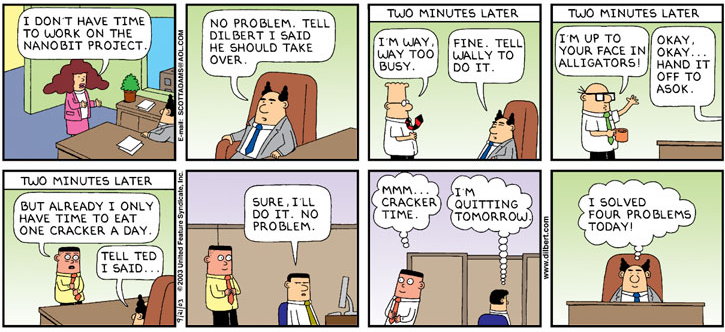
\includegraphics[width=\linewidth]
	  {bilder/comics/dilbert.png}    \end{center}
%	\end{wrapfigure}
\begin{multicols}{2}
%%% Local Variables: 
%%% mode: latex
%%% TeX-master: "../../1-te"
%%% End: 
